%% LyX 2.2.4 created this file.  For more info, see http://www.lyx.org/.
%% Do not edit unless you really know what you are doing.
\documentclass[english]{article}
\usepackage[T1]{fontenc}
\usepackage[latin9]{inputenc}
\usepackage{geometry}
\geometry{verbose,lmargin=4.5cm,rmargin=4.5cm}
\usepackage{color}
\usepackage{babel}
\usepackage{float}
\usepackage{textcomp}
\usepackage{url}
\usepackage{graphicx}
\usepackage[unicode=true,pdfusetitle,
 bookmarks=true,bookmarksnumbered=false,bookmarksopen=false,
 breaklinks=true,pdfborder={0 0 1},backref=false,colorlinks=false]
 {hyperref}
\usepackage{breakurl}

\makeatletter
%%%%%%%%%%%%%%%%%%%%%%%%%%%%%% User specified LaTeX commands.
%\usepackage[T1]{fontenc}
\usepackage{charter}
\usepackage[table]{xcolor}
\usepackage{amsmath}
\newcommand{\mathA}[1]{{\operatorname{#1}}}
\newcommand{\mathB}[1]{{\operatorname{\mathit{#1}}}}


% Luis Garreta defs
\renewcommand{\textrightarrow}{$\rightarrow$}

\newcommand{\blue}[1]{{\textcolor{blue}{#1}}}

\usepackage[font=scriptsize,labelfont=bf]{caption}

%\pagecolor{yellow!30}
\usepackage[colorinlistoftodos]{todonotes}
\setlength{\marginparwidth}{4.3cm}
\newcommand{\lc}[1]{\todo[size=\small,color=red!20!white]{#1}}
\newcommand{\ic}[1]{\todo[size=\small,color=green!20!white]{#1}}
\newcommand{\pr}[1]{\todo[size=\small,color=blue!20!white]{#1}}

\makeatother

\usepackage{listings}
\renewcommand{\lstlistingname}{Listing}

\begin{document}

\title{MultiGWAS: A tool for GWAS analysis on tetraploid organisms by integrating four GWAS software}
\maketitle
\begin{abstract}
\textbf{Summary:} The Genome-Wide Association Studies (GWAS) are essential to determine the association between genetic variants across individuals. One way to support the results is by using different tools to validate the reproducibility of the associations. Currently, software for GWAS in diploids is well-established but for polyploids species is scarce. Each GWAS software has its characteristics, which can cost time and effort to use them successfully. Here, we present MultiGWAS, a tool  perform GWAS analysis in tetraploid organisms by executing in parallel and integrating the results from four existing GWAS  packages: two available for polyploids (GWASpoly and SHEsis) and two frequently used for diploids (PLINK and TASSEL). The tool deals with all the elements of the GWAS process in the four packages, including (1) Genomica data management from different input formats (2) Data cleaning using different control quality filters, (3) Data conversion for package file formats (4) GWAS Execution in the for packages using two GWAS models, the full model with control for population structure and individual relatedness and the Naive model without any control (5) Summary statististicswith tables and plots describing intuitively the significant association found by \textcolor{red}{both each one and across four packages,} \textcolor{red}{which helps users to check for false-positive or false-negative results.}
\end{abstract}

\section{Introduction}

The \textcolor{blue}{Genome-wide association studies (GWAS) are} used to identify which variants through the whole genome of a large number of individuals are associated with a specific trait (\cite{cantor2010prioritizing,begum2012comprehensive}). This methodology started with humans and several model plants, such as rice, maize, and \emph{Arabidopsis} (\cite{lauc2010genomics,tian2011genome,cao2011whole,korte2013advantages,han2013sequencing}). Because of the advances in the next-gen sequencing technology and the decline of the sequencing cost in recent years, there is an increase in the availability of genome sequences of different organisms at a faster rate (\cite{ekblom2011applications,ellegren2014genome}). Thus, the GWAS is becoming the standard tool to understand the genetic bases of either ecological or economic phenotypic variation for both model and non-model organisms. This increment in GWAS includes complex species such as polyploids (Fig. \ref{GWASpolyploids}) (\cite{ekblom2011applications,santure2018wild}).

% Figure timelines articles
\begin{figure}[H]
\begin{centering}
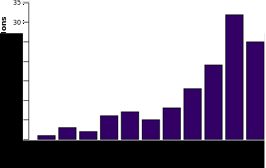
\includegraphics{images/01_paper-GWASpolyploids-PubMed}
\par\end{centering}
\centering{}\caption{Timeline for articles reported for GWAS studies on polyploid species in PubMed. We present data for completed years.\label{GWASpolyploids}}
\end{figure}

The GWAS for polyploid species has three related challenges. First, as all GWAS, we should replicate the study as a reliable method to validate the results and recognize real associations. This replication involves finding the same associations either in several replicates from the study population using the \lc{Me confunde al hablar de software y tools} same software or testing different GWAS tools among the same study population. \lc{\textquotedbl{}The latter approach...\textquotedbl{}} This approach involved the use of different parameters, models, or conditions, to test how consistent the results are (\cite{De2014,Pearson2008}). However, the performance of different \lc{Software or tools ??}GWAS software could affect the results. For example, the threshold $pvalue$ for SNP significance change through four GWAS software (i.e., PLINK, TASSEL, GAPIT, and FaST-LMM) when sample size varies (\cite{Yan2019}). It means that well-ranked SNPs from one package can be ranked differently in another.

Second, although there are many GWAS software available to repeat the analysis under different conditions (\cite{Gumpinger2018}), most of them are designed exclusively for the diploid data matrix (\cite{Bourke2018}). Therefore, it is often necessary to \textquotedbl{}diploidizing\textquotedbl{} the polyploid genomic data in order to replicate the analysis.

Third, there are very few tools focused on the integration of several GWAS software, to make comparisons under different parameters and conditions across them. As far as we know, there is only two software with this service in mind, such as iPAT and easyGWAS.

\textbf{The} iPAT allows running in a graphic interface three well-known command-line GWAS software such as GAPIT, PLINK, and FarmCPU (\cite{Zhang2018}) . However, the output from each package is separated. On the other hand, the easyGWAS allows running a GWAS analysis on the web using different algorithms. This analysis could run independently of both the computer capacity and operating system. However, it needs either several datasets available or a dataset with a large number of individuals to make replicates in order to compare among algorithms. Moreover, the output from different algorithms is separated (\cite{Grimm2017}). Thus, for both software iPAT and easyGWAS, the integrative and comparative outputs among software or algorithms are missing.

\textcolor{red}{To solve all the three challenges above, \lc{To solve the above three challenges?}} we developed the MultiGWAS tool that performs GWAS analyses for tetraploid species using four software in parallel. Our tool include GWASpoly (\cite{Rosyara2016}) and the SHEsis tool (\cite{Shen2016}) that accept polyploid genomic data, and PLINK (\cite{Purcell2007}) and TASSEL (\cite{Bradbury2007}) with the use of a \textquotedbl{}diploidized\textquotedbl{} genomic matrix. The tool deals with \textcolor{blue}{input file formats, data preprocessing, search for associations by running} four GWAS tools in parallel, and \textcolor{blue}{creation of} comparative reports from the output of each software to help the user to decide more intuitively the true or false associations.

\section{Methods}

The MultiGWAS tool has three main consecutive steps: the adjustment, the multi analysis, and the integration (Fig. \ref{fig:Pipeline}). In the adjustment step, MultiGWAS processes the configuration file, cleans and filters the genotype and phenotype, and \textquotedbl{}diploidize\textquotedbl{} the genomic data. Then, during the multi analysis, each GWAS tool runs in parallel. Finally, in the integration step, the MultiGWAS tool scans the output files from the four packages (i.e., GWASPoly, SHEsis, PLink, and TASSEL). 

MultiGWAS generates a summary of all results that contains the following tabular and graphical visualizations: score tables with detailed information of associations, shared SNPs visualization using Venn diagrams, SNP profiles using heatmaps, associations visualizations using Manhattan and QQ plots, and chromosomes vs SNP visualizations using chord diagrams. 

% Figure MultiGWAS stages

\begin{figure}
\centering{}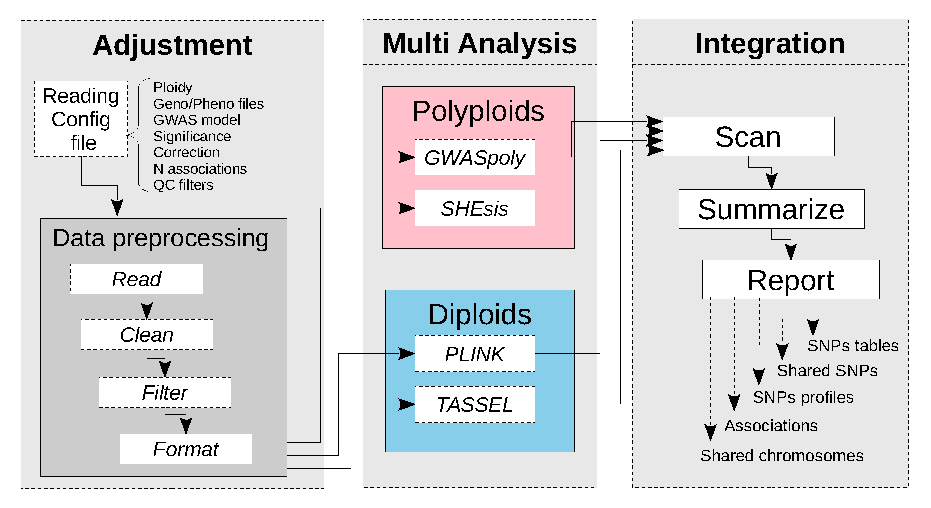
\includegraphics[width=12cm]{images/paper-multiGWAS-flowchart-stages} \caption{\textbf{MultiGWAS flowchart has three steps: adjustment, multi analysis, and integration.} The first step deals with input data management, reading the configuration file, \textcolor{blue}{reading and preprocessing the input genomic data} (genotype and phenotype). The second step deals with GWAS analysis, configuring and running the four packages in parallel. And the third step deals with summarizing and reporting results using different tabular and graphical visualizations.\label{fig:Pipeline}}
\end{figure}


\subsection{Adjustment stage}

MultiGWAS takes as input a configuration file where the user specifies the genomics data and the parameters used by the four tools. Once the configuration file is read and processed, the genomic data files (genotype and phenotype) are then cleaned, filtered, and checked for data quality. The output of this stage corresponds to the inputs for the four programs at the Multi Analysis stage.

%genotype/phenotype filenames, genome-wide significance threshold, multiple testing correction methods, GWAS model, number of associations to be reported, and TRUE or FALSE whether to use quality control (QC) filters or not. 

\subsubsection{Reading configuration file\label{section-Reading-configuration-file}}

The configuration file includes the following settings that we briefly describe:% (1) Input genotype and phenotype file names (2) GWAS model, (3) Significance threshold, (4) Correction (5) Quality Control (QC) filters and (6) number of associations to report. 

\paragraph{Ploidy:}

Numerical value for the ploidy level of the genotype, currently MultiGWAS supports diploids and tetraploids genotypes (2: for diploids, 4: for tetraploids).

\paragraph{Genotype and phenotype input files:}

\textcolor{blue}{MultiGWAS uses two input files, one for the genotype and one for the phenotype. Genotype data can be input in three different formats, including a matrix format (Fig. \ref{fig:File-Formats}.a), a GWASpoly format (\cite{Rosyara2016}) (Fig. \ref{fig:File-Formats}.b), and Variant Call Format (VCF) (Fig.\ref{fig:File-Formats}.c) which is transformed into GWASpoly format using NGSEP 4.0.2 (\cite{Duitama2019}). The phenotype file contains only one trait with the first column for the sample names and the second column for the trait values (Fig. \ref{fig:File-Formats}.c).}

\begin{figure}[H]
\begin{centering}
\includegraphics{images/03_paper-input-files} 
\par\end{centering}
\caption{\textbf{\scriptsize{}Examples of MultiGWAS input file formats}{\scriptsize{}. }\textcolor{blue}{\scriptsize{}Figures a, b and c show examples of genotypes, while figure d shows an example of a phenotype. }\textbf{\textcolor{blue}{\scriptsize{}a}}\textcolor{blue}{\scriptsize{}. Genotype file in matrix format containing in the first column the marker names and in the following columns the marker data of the samples coded in \textquotedbl{}ACGT\textquotedbl{} format (e.g. AAGG, CCTT for tetraploids, AG, CT for diploids). }\textbf{\textcolor{blue}{\scriptsize{}b}}\textcolor{blue}{\scriptsize{}. Genotype file in GWASpoly format adding the chromosome and marker position to the matrix format.}{\scriptsize{} }\textbf{\scriptsize{}c}{\scriptsize{}. Genotype file in VCF format with metadata (first two lines) and header line. The following lines contain genotype information of the samples for each position. VCF marker data can be encoded as simple genotype calls (GT format field, e.g., 0/0/1/1 for tetraploids or 0/1 for diploids) or using the NGSEP custom format fields (\cite{Duitama2019}): ACN, ADP or BSDP. }\textbf{\scriptsize{}d}{\scriptsize{}. Phenotype file in a matrix format with column headers and sample names followed by their trait values. Both GWASpoly genotype and phenotype files are in CSV (Comma Separated Values format).}}
\label{fig:File-Formats}\protect 
\end{figure}


\paragraph{GWAS model:}

MultiGWAS is designed to work with quantitative phenotypes and can run GWAS analysis using two types of statistical models that we have called \emph{full} and \emph{naive} models. The \emph{full model} is known in the literature as the Q+K model (\cite{Yu2006}) and includes a control for structure (Q) and relatedness between samples (K). In contrast, the \emph{naive model} does not include any type of correction. Both models are linear regression approaches, and each one of the four GWAS packages used in MultiGWAS has some variations of those models. The \emph{naive} is modeled with Generalized Linear Models (GLMs, Phenotype + Genotype), and the \emph{full} is modeled with Mixed Linear Models (MLMs, Phenotype + Genotype + Structure + Kinship). The default model used by MultiGWAS is the \emph{full model} (Q+K) (\cite{Yu2006}), following the equation:

\[
y=X\beta+S\alpha+Q\nu+Z\mu+e
\]

In this equation, the $y$ is the vector of observed phenotypes. Moreover, the $\beta$ is a vector of fixed effects other than SNP or population group effects, the $\alpha$ is a vector of SNP effects (Quantitative Trait Nucleotides), the $\nu$ is a vector of population effects, the $\mu$ is a vector of polygene background effects, and the $e$ is a vector of residual effects. Besides, $Q$, modeled as a fixed effect, refers to the incidence matrix for subpopulation covariates relating $y$ to $\nu$, and $X$, $S$ and $Z$ are incidence matrices of 1s and 0s relating $y$ to $\beta$, $\alpha$ and $\mu$, respectively.

\paragraph{Genome-wide significance: }

GWAS searches SNPs associated with the phenotype in a statistically significant manner. A threshold or significance level $\alpha$ is specified and compared with the \emph{p-value} derived for each association score. Standard significance levels are 0.01 or 0.05 (\cite{Gumpinger2018,Rosyara2016}), and MultiGWAS uses an $\alpha$ of 0.05 for the four GWAS packages. However, in GWASpoly and TASSEL, which calculates the SNP effect for each genotypic class using different gene action models (see ``Multi analysis stage''), the threshold is adjusted according to each of those two packages. Therefore, the number of tested markers\emph{ }may be different in each model (see below), impacting the \emph{p-value} thresholds.

\paragraph{Multiple testing correction:}

Due to the massive number of statistical tests performed by GWAS, it is necessary to perform a correction method for multiple hypothesis testing and adjusting the \emph{p-value} threshold accordingly. Two standard methods for multiple hypothesis testing are the false discovery rate (FDR) and the Bonferroni correction. The latter is the default method used by MultiGWAS, which is one of the most rigorous methods. However, instead of adjusting the \emph{p-values,} MultiGWAS adjust the threshold below which a \emph{p-value} is considered significant. That is $\alpha/m$, where $\alpha$ is the significance level and \emph{m }is the number of tested markers from the genotype matrix.

\paragraph{Number of reported associations: }

Criticism has arisen, considering only statistically significant associations as possible correct associations (\cite{Thomson2011,Kaler2019}). Many low \emph{p-value} associations, closer to being significant, are discarded due to the stringent significance levels, which consequently increases the number of false negatives. To avoid this problem, MultiGWAS provides the option to specify the number of best-ranked associations (lower \emph{p-values}), adding the corresponding \emph{p-value} to each association found. In this way, it is possible to enlarge the number of results, and their replicability across the different programs. Nevertheless, the report displays each association with its corresponding \emph{p-value}.

%  We present the resultant associations in different tables and graphics reported by MultiGWAS (see Figure \ref{fig:-View-Shared-SNPs}). 

\paragraph{Quality control filters:}

A control step is necessary to check the input data for the genotype or phenotype errors or poor quality that can lead to spurious GWAS results. MultiGWAS provides the option to select and define thresholds for the following filters that control the data quality: Minor Allele Frequency (MAF), individual missing rate (MIND), SNP missing rate (GENO), and Hardy-Weinberg threshold (HWE): 
\begin{itemize}
\item \textbf{MAF of }\textbf{\emph{x:}} filters out SNPs with minor allele frequency below \emph{x} (default 0.01); 
\item \textbf{MIND of }\textbf{\emph{x:}} filters out all individuals with missing genotypes exceeding \emph{x}{*}100\% (default 0.1); 
\item \textbf{GENO of }\textbf{\emph{x:}} filters out SNPs with missing values exceeding \emph{x}{*}100\% (default 0.1); 
\item \textbf{HWE of }\textbf{\emph{x:}} filters out SNPs with a \emph{p-value} below the \emph{x} threshold in the Hardy-Weinberg equilibrium exact test.(for diploids)

%\ic{Comentario de Andr�s: una pregunta m�s metodol�gica tiene que ver con HWE. en poliploides la hetrocigosidad está inflada, y por ello desviar��a en HWE si esta se calcula tradicionalmente. por ello, son las fercuencias genotípicas esperadas calculadas para poliplodes? i.e. (p+q) elevado a la n donde n es la ploid�a}

\end{itemize}
MultiGWAS does the MAF filtering, and uses the PLINK package (\cite{Gumpinger2018}) for the other three filters: MIND, GENO, and HWE.

\paragraph{GWAS tools:}

List of names of the four GWAS software to run and integrate into MultiGWAS analysis. They are GWASpoly and SHEsis (designed for polyploid data), and PLINK and TASSEL (designed for diploid data).

\subsubsection{Data preprocessing}

Once the configuration file is processed, the genomic data is read and cleaned by selecting individuals present in both genotype and phenotype. Then, MultiGWAS removes individuals and SNPs with poor quality following the previous selected quality-control filters and their thresholds,

At this point, the format \textquotedbl{}ACGT\textquotedbl{} suitable for the polyploid software GWASpoly and SHEsis, is \textquotedbl{}diploidized\textquotedbl{} for PLINK and TASSEL. The homozygous tetraploid genotypes are converted to diploid thus: AAAA\textrightarrow AA, CCCC\textrightarrow CC, GGGG\textrightarrow GG, TTTT\textrightarrow TT. Moreover, for tetraploid heterozygous genotypes, the conversion depends on the reference and alternate alleles calculated for each position (e.g., AAAT \textrightarrow AT, ... ,CCCG\textrightarrow CG).

After this process, MultiGWAS converts the genomic data, genotype, and phenotype datasets to the specific formats required for each of the four GWAS packages. 

\subsection{Multi analysis stage}

MultiGWAS runs in parallel using two types of statistical models specified in the parameters file, the Full model (Q+K) and Naive (i.e., without any control) \cite{Sharma2018}. The Full model (Q+K) controls for both population structure and individual relatedness. For population structure, MultiGWAS uses the Principal Component Analysis (PCA) and takes the top \textcolor{blue}{five} PC as covariates. For relatedness, \textcolor{blue}{MultiGWAS} uses kinship matrices that TASSEL and GWASpoly calculated separately, and for PLINK and SHEsis, \textcolor{blue}{relatedness depends of kinship coefficients calculated with the PLINK 2.0 built-in algorithm \cite{Chang2015}. }

%\subsubsection{Tools}We have selected four GWAS software tools to be integrated in our multiGWAS tool, two designed specifically for polyploid species as many important crops are polyploids: GWASpoly \cite{Rosyara2016} and SHEsis \cite{Yong2006}, and another two designed for diploids species and extensively used in humans and plants: PLINK \cite{Purcell2007,Chang2015} and TASSEL \cite{Bradbury2007}, respectively.

As MultiGWAS implements two types of GWAS analysis, naive and full, each tool is called in two different ways. %The naive without any additional parameter, but the full with two parameters that take into account for population structure (Q) and relatedness (K) to prevent false associations.

\subsubsection{GWASpoly}

GWASpoly \cite{Rosyara2016} is an R package designed for GWAS in polyploid species used in several studies in plants \cite{Berdugo2017,Ferrao2018,Sharma2018,Yuan2019}. GWASpoly uses a Q+K linear mixed model with biallelic SNPs that account for population structure and relatedness. \textcolor{blue}{Also, to calculate the SNP effect for each genotypic class, GWASpoly provides eight gene action models: general, additive, simplex dominant alternative, simplex dominant reference, duplex dominant alternative, and duplex dominant. As a consequence, the number of statistical test performed can be different in each action model and so thresholds below which the }\textcolor{blue}{\emph{p-values}}\textcolor{blue}{{} are considered significant.}

MultiGWAS is using GWASpoly version 1.3, \textcolor{blue}{employing all gene action models to find associations and repoting the top }\textcolor{blue}{\emph{N }}\textcolor{blue}{best-ranked (the SNPs with lowest }\textcolor{blue}{\emph{p-values)}}\textcolor{blue}{, where }\textcolor{blue}{\emph{N}}\textcolor{blue}{{} is defined by the user in the input configuration file.} The \emph{full }model used by GWASpoly includes the population structure and relatedness, which are estimated using the first five principal components and the kinship matrix, respectively, both calculated with the GWASpoly built-in algorithms.

\subsubsection{SHEsis}

SHEsis is another program designed for polyploid species that includes single locus association analysis, among others. It is based on a linear regresion model, and it has been used in some studies of animals and humans \cite{Qiao2015,Meng2019}.

MultiGWAS is using the version 1.0 which does not take account for population structure or relatedness, however MultiGWAS externally estimates relatedness for SHEsis by excluding individuals with cryptic first-degree relatedness using the algorithm implemented in PLINK 2.0 (see below).

\subsubsection{PLINK}

PLINK is one of the most extensively used programs for GWAS in diploids species. It was developed for humans but it is applicable to any species \cite{Power2016}. PLINK includes a range of analysis, including univariate GWAS using two-sample tests and linear regression models.

MultiGWAS is using two versions of PLINK: 1.9 and 2.0. Linear regression from PLINK 1.9 is used to achieve both types of analysis, naive and full. For the full analysis, population structure is estimated using the first five principal components calculated with the PLINK 1.9 built in algorithm. But relatedness is estimated from the kinship coefficients calculated with the PLINK 2.0 built in algorithm, removing the close relatives or individuals with first-degree relatedness.

\subsubsection{TASSEL}

TASSEL is another common GWAS program based on the Java software. It was developed for maize and it has been used in several studies in plants \cite{Alvarez2017,Zhang2018}, but like PLINK, it is applicable to any species. For association analysis, TASSEL includes the general lineal model (GLM) and mixed linear model (MLM) that accounts for population structure and relatedness. \textcolor{blue}{And, in the same manner that GWASPoly, TASSEL provides three gene action models to calculate the SNP effect of each genotypc class: general, additive, and dominant, and so the significance threshold depends of each action model.}

MultiGWAS is using TASSEL 5.0, \textcolor{blue}{with all gene action models used to find the }\textcolor{blue}{\emph{N }}\textcolor{blue}{best-ranked associations and reporting the top }\textcolor{blue}{\emph{N }}\textcolor{blue}{best-ranked associations (SNPs with lowest }\textcolor{blue}{\emph{p-values)}}\textcolor{blue}{.} Naive GWAS is achieved by the GLM, and full GWAS is achieved by the MLM with two parameters: population structure that uses the first five principal components, and relatedness that uses the kinship matrix with centered IBS method, both calculated with the TASSEL built-in algorithms. 

\subsection{Integration stage.}

\color{blue}

The outputs resulting from the four GWAS packages are scanned and processed to identify both significant and best-ranked associations with \emph{p-values} lower than and close to a significance threshold, respectively. 

\subsubsection{Calculation of \emph{p-values }and significance thresholds}

GWAS packages compute \emph{p-value }as a measure of association between each individual SNP and the trait of interest. The SNPs are considered statistically significant, and so possible true associations, when their \emph{p-value }drops below a predefined significance threshold. But, most GWAS packages compute differently \emph{p-values} with the possibility to compute them too high or too low. If \emph{p-values} are too high, then it would lead to false negatives or SNPs with true associations with the phenotype but that does not reach the significance threshold. Conversely, if \emph{p-values} are too low, then it would lead to false positives or SNPs with false associations with the phenotype but that reaches the significance threshold.

To overcome these difficulties, in the case of too high \emph{p-values}, MultiGWAS identifies and reports both significant and best-ranked associations (the ones closer to being statistically significant). Whereas, in the case of too low \emph{p-values}, MultiGWAS provides two methods for adjusting \emph{p-values} and significance threshold: the false discovery rate (FDR) that adjust \emph{p-values, }and the Bonferroni correction, that adjusts the threshold.

By default, MultiGWAS uses the Bonferroni correction in which the significance threshold is adjusted as $\alpha/m$, where $\alpha$ is the significance level defined by the user in the configuration file, and $m$ is the number of tested markers in the GWAS study. However, the significance threshold can be different for each GWAS package as some of them use several action models to calculate the SNP effect of each genotypic class. For both PLINK and SHEsis packages, which use only one model, $m$ is equal to the total number of SNPs, but for both GWASpoly and TASSEL packages, which use eight and three gene action models, respectively, $m$ is equal to the number of test performed in each model, which is different between models.

\color{black}

\subsubsection{Selection of significant and best-ranked associations}

MultiGWAS selects two groups of associations from the results of each GWAS package: statistically significant and best-ranked. The latter equally important to the former as they are associations with lowest \emph{p-values} not reaching the significance threshold but representing interesting associations for further analysis (possible false negatives). 

The significant associations are selected from the ones with \emph{p-values} falling below a significant threshold, calculated for each GWAS package; and the best-ranked associations are selected as the closest \emph{N} to being statistically significant, with \emph{N} defined by the user in the configuration file.

The selection of these groups takes into account whether the GWAS package uses only one gene action model, as PLINK and SHEsis do, or uses several ones, as GWASpoly and TASSEL do. In the first case, there is only one resulting set of associations and the selection is straighforward, as described above. However, in the second case, there are several resulting sets of associations, one for each model, and MultiGWAS selects both groups of associations by choosing the gene action model with the highest number of shared SNPs and with the inflation factor closest to one, according to the following equation:

\[
score(M_{i})=\frac{\sum\limits _{j=1}^{k}{\textstyle sharedSNPs(M_{i},M_{j})}}{k*N}+1-|1-\lambda(M_{i})|
\]

where $score(M_{i})$ is the score for the gene action model $M_{i}$, with $i$ from $1..k$, for a GWAS package with $k$ gene action models; $sharedSNPs(M_{i},M_{j})$ is the number of shared SNPs between models $M_{i}$ and $M_{j}$; $N$ is the number of closest SNPs to being statistically significant, as it was described above; and $\lambda(M_{i})$ is the inflation factor for the model $M_{i}$.

The score is high when a model $M_{i}$ both identifies a high number of shared SNPs and has an inflation factor $\lambda$ close to 1. Conversely, the score is low when the model $M_{i}$ both identifies a small number of shared SNPs and has an inflation factor $\lambda$ either low (close to 0) or high ($\lambda>2$ ). In any other case, the score is balanced between the number of shared SNPs and the inflation factor.

\subsubsection{Integration of results}

% Figure several reports

\begin{figure}
\includegraphics[width=12cm]{images/paper-methodologies-all-plots} \caption{\textbf{\textcolor{blue}{Reports presented by MultiGWAS}}\textcolor{blue}{.} For each tool, first a QQ plot that \textcolor{blue}{assesses} the resultant p-values. Second, a Manhattan plot for each tool with two lines, blue and red, respectively, is the lower limit for the best ranked and significative SNPs. We present two Venn diagrams, one for the significative SNPs and one for N best-ranked SNPs of each tool. We show the results for GWAspoly, PLINK, TASSEL, and SHEsis in red, green, yellow, and blue, respectively. For each SNP that is in the intersection; thus, that is predicted by more than one tool we provide SNP profile. \textcolor{blue}{Chord diagrams for SNPs by chromosome showing how the strongest associations are mostly found on few chromosomes. And we also present tabular summaries with details of significant and best-ranked associations. }\label{fig:Reports} }
\end{figure}

At this stage, \textcolor{blue}{MultiGWAS integrates} the results to evaluate reproducible results among tools (Fig. \ref{fig:Reports}). But, it still reports a summary for the results of each tool: 
\begin{itemize}
\item A Quantile-Quantile (QQ) plots for the resultant \emph{p-values} of each tool and the corresponding \textcolor{blue}{inflation factor} $\lambda$ to asses the degree of the test statistic inflation. 
\item A Manhattan plot of each tool with two lower thresholds, one for the best-ranked SNPs, and another for the significant SNPs. 
\end{itemize}
To present the replicability, we use two sets: (1) the set of all the significative SNPs provided by each tool and (2) the set of all the best-ranked SNPs. For each set, we present a Venn diagram that shows SNPs predicted exclusively by one tool and intersections that help to identify the SNPs predicted by one, two, three, or all the tools. In addition, we provide detailed tables for the two sets.

For each SNP identified more than once, we provide what we call the SNP profile. That is a heat diagram for a specific SNP, where each column is a genotype state AAAA, AAAB, AABB, ABBB, and BBBB. And each row corresponds to a sample. Samples with close genotypes form together clusters. Thus to generate the clusters, we do not use the phenotype information. However, we present the phenotype information in the figure as the color. This figure visually provides information regarding genotype and phenotype information simultaneously for the whole population. We present colors as tones between white and black for color blind people.

MultiGWAS generates a report, one document with the content previously described. Besides, there is a folder with the individual figures just in case the user needs one. \textcolor{blue}{In the supplementary information, we include a report and a description of the report content (Supplementary Material 1)}

\textcolor{blue}{In the following section, we present the results of the functionality of the tool applied on a diversity panel of a tetraploid potato, genotyped and phenotyped as part of the USDA-NIFA Solanaceae Coordinated Agricultural Project (SolCAP) \cite{Hirsch2013}.}

\pr{infomraciOn suplementary con reporte completo y figuras. Y explicaciOn del reporte}


\section{Results}

Most of the GWAS packages used by MultiGWAS are based on a linear regression approaches, but they often produce dissimilar association results for the same input. For example, computed \emph{p-values }for the same set of SNPs are different between packages; SNPs with significant \emph{p-values} for one package may be not significant for the others; or well-ranked SNPs in one package may be ranked differently in another. 

To alleviate these difficulties, MultiGWAS produces five types of outputs using different graphics and tabular views, these outputs are intended to help users to compare, select, and interpret the set of possible SNPs associated with a trait of interest. The outputs include: 
\begin{itemize}
\item Manhattan and Q-Q plots to show GWAS associations. 
\item Venn diagrams to show associations identified by single or several tools.
\item Heat diagrams to show the genotypic structure of shared SNPs.
\item Chord diagrams to show shared SNPs by chromosomes.
\item Score tables to show detailed information of associations for both summary results from MultiGWAS and particular results from each GWAS package
\end{itemize}
\textcolor{blue}{The complete reports generated by MultiGWAS are shown in the supplementary information at~ \url{https://github.com/agrosavia-bioinformatics/multiGWAS-Supplementary}.}


\subsection{Manhattan and QQ plots for GWAS associations }

MultiGWAS uses classical Manhattan and Quantile\textendash Quantile plots (QQ plots) to visualize the results of each package. In both plots, the points are the SNPs and their p-values are transformed into scores like $-log_{10}(\mathB{p-values})$ (see Fig. \ref{fig:view-qqmanhattan}). The Manhattan plot shows the strength of association of the SNPs (y-axis) distributed at their genomic location (x-axis), so the higher the score, the stronger the association. While the QQ plot compares the expected distribution of \emph{p-values} (y-axis) with the observed distribution (x-axis).. \lc{Corregido: "among packages" y cita de polygenic traits}\ic{Revisar si esto del color verde es correcto "shared among all packages". Tambi�n revisar si est� bien dicho lo de la comparaci�n entre pocos genes y muchos genes. No se si sea necesario cuantificar la desviaci�n. Originalmente se cuantificaba pero era confuso}\lc{Ya est�}\ic{La leyenda debe incluir tambi�n la descripci�n de qu� significa las lineas rojas, azules y los puntos verdes}

MultiGWAS adds distinctive marks to both plots to identify different types of SNPs: (a) In the Manhattan plots, the significant SNPs are above a red line and the best-ranked SNPs are above a blue line. In addition, \textcolor{blue}{SNPS shared between packages are colored green} (See Fig. \ref{fig:Table-Shared-SNPs}.b). (b) In the QQ plots, a red diagonal line indicates the expected distribution under the null hypothesis of no association of SNPs with the phenotype, both distributions should coincide, and most SNPs should lie on the diagonal line. \textcolor{blue}{Deviations for a large number of SNPs may reflect inflated }\textcolor{blue}{\emph{p-values }}\textcolor{blue}{due to population structure or cryptic relatedness. But, it is also expected that few SNPs deviate from the diagonal for a truly polygenetic trait (\cite{Power2016}).}

\begin{figure}[H]
\begin{centering}
\includegraphics{images/paper-manhattan-QQ-plots}
\par\end{centering}
\caption{\textbf{\textcolor{blue}{Associations in the tetraploid potato dataset.}}\textcolor{blue}{{} MultiGWAS shows the associations identified by the four GWAS packages using Manhattan and QQ plots. In the case of the tetraploid potato, several SNPs are observed to be shared between the four packs (green dots). The best-ranked SNPs are above the blue line, but only GWASpoly and SHEsis identified significant associations (SNPs above the red line). However, the inflation factor given by SHEsis is too high ($\lambda=3.5$, at the top of the QQ plot), which is observed by the high number of SNPs deviating from the red diagonal of the QQ plot. \label{fig:view-qqmanhattan}}}
\end{figure}


\subsection{Tables and Venn diagrams for single and shared SNPs}

MultiGWAS provides tabular and graphic views to report in an integrated way both the best-ranked and significant SNPs identified by the four GWAS packages (see Figure \ref{fig:Table-Shared-SNPs}). Both \emph{p-values} and significance levels have been scaled as $-log_{10}(\mathB{p-value})$ to give high scores to the best statistically evaluated SNPs.

First, best-ranked SNPs correspond to the top-scored \emph{N} SNPs, wheter they were assesed significant or not by its package, and with\emph{ N} defined by the user in the configuration file. These SNPs are shown both in a SNPs table (Figure \ref{fig:Table-Shared-SNPs}.a) and in a Venn diagram (Figure \ref{fig:Table-Shared-SNPs}.b). The table lists them by package and sorts by decreasing score, whereas the Venn diagram shows them emphasizing if they were best-ranked either in a single package or in several at once (shared). And second, the significant SNPs correspond to the ones assesed statistically significant by each package, they are shown in a Venn diagram (Figure \ref{fig:Table-Shared-SNPs}.c), and they are also shown in the SNPs table, marked with significance TRUE (T) in the table of the Figure\ref{fig:Table-Shared-SNPs}.a.

\begin{figure}[H]
\begin{centering}
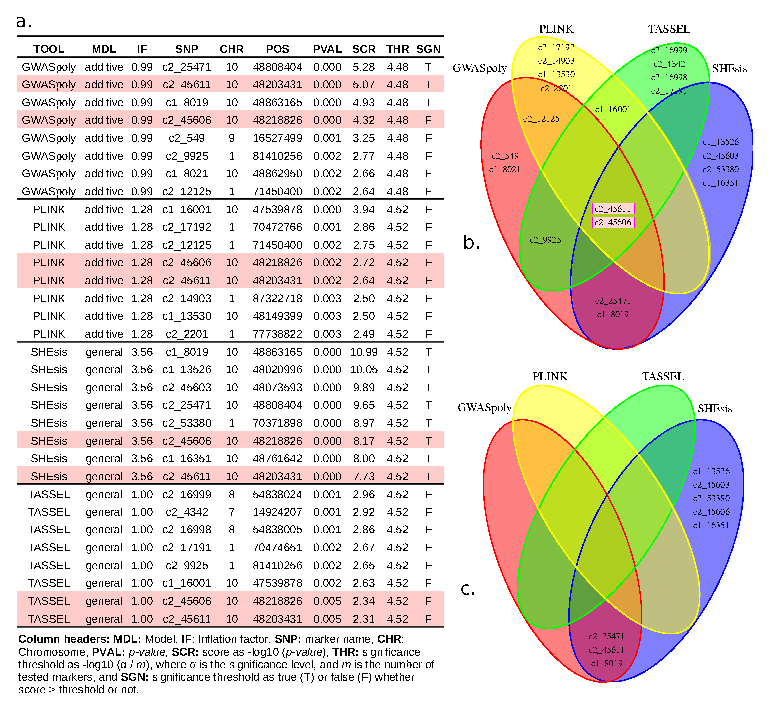
\includegraphics{images/paper-table-venn-best}
\par\end{centering}
\caption{\textbf{Shared SNPs Views. }Tabular and graphical views of SNP associations identified by one or more GWAS packages (shared SNPs). SNPs identified by all packages are marker with red background in all figures \textbf{(a)} Table with details of the N=9 best-ranked SNPs from each GWAS package. Each row corresponds to a single SNP and the 9 columns are: tool name, model used by the tool, genomic control factor (inflation factor), SNP name, chromosome, position in the genome, \emph{p-value}, score as $-log_{10}(\mathB{p-value})$, significance threshold as $-log_{10}(\alpha/m)$ where $\alpha$ is the significance level and $m$ is the number of tested markers, and significance as true (T) or false (F) whether score > threshold or not. \textbf{(b)} Venn diagram of the N=9 best-ranked SNPs. SNPs identified by all packages are located in the central intersection. Other SNPs identified by more than one packages are located in both upper central and lower central intersections. \textbf{(c)} Venn diagram of the significant SNPs (score > threshold). \label{fig:Table-Shared-SNPs}}
\end{figure}

 

\subsection{Heat diagrams for structure of shared SNPs}

MultiGWAS creates a two-dimensional representation, called SNP profile, to visualize each trait by individuals and genotypes as rows and columns, respectively (Figure \ref{fig:SNP-profiles}). At the left, the individuals are grouped in a dendrogram by their genotype. At the right, there is the name or ID of each individual. At the bottom, the genotypes are ordered from left to right, starting from the major to the minor allele (i.e., AAAA, AAAB, AABB, ABBB, BBBB). At the top, there is a description of the trait based on a histogram of frequency (top left) and by an assigned color for each numerical phenotype value using a grayscale (top right). Thus, each individual appears as a colored line by its phenotype value on its genotype column. For each column, there is a solid cyan line with the mean of each column and a broken cyan line that indicates how far the cell deviates from the mean.

Because each multiGWAS report shows one specific trait at a time, the histogram and color key will remain the same for all the best-ranked SNPs.

\begin{figure}[H]
\begin{centering}
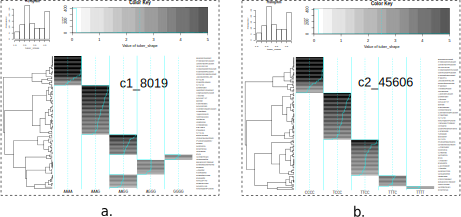
\includegraphics{images/paper-heat-maps}
\par\end{centering}
\caption{\textbf{\scriptsize{}SNP profiles. }{\scriptsize{}SNP profiles for two of the best-ranked significant SNPs shown in the figure \ref{fig:Table-Shared-SNPs}.b. (a) SNP c2\_45606 best-ranked by the four packages (central intersection of the Venn diagram Figure \ref{fig:Table-Shared-SNPs}.b) (b) SNP c1\_8019 best-ranked by the two tetraploid packages (Figure \ref{fig:Table-Shared-SNPs}.b), and also identified as significant by the same packages (at the bottom of the Figure \ref{fig:Table-Shared-SNPs}.a). \label{fig:SNP-profiles}}}
\end{figure}


\subsection{Chord diagrams for SNPs by chromosome}

The chord diagrams visualize the location across the genome of the best-ranked associated SNPs shared among the four packages and described in the table \ref{fig:Table-Shared-SNPs}.a. Thus, in the case of the tetraploid potato, we found that they are located mostly in chromosomes 1 and 10 (Figure \ref{fig:Chord-diagrams}.a). This visualization complements the manhattan plots from each GWAS package (Figure \ref{fig:Chord-diagrams}.b).

\begin{figure}
\begin{centering}
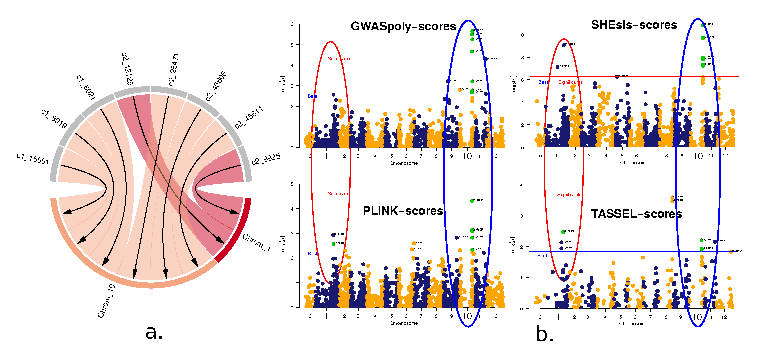
\includegraphics{images/08_paper-chord-manhattans} 
\par\end{centering}
\caption{\textbf{The position of best-ranked SNPs across chromosomes using two different visualizations.} \textbf{(a)} Chord diagram showing that best-ranked SNPs located in chromosomes 1 and 10. The SNPs are at the top and the chromosomes at the bottom. The arrows connect the SNPs with their position in the chromosomes. \textbf{(b)} Manhattan plots from each GWAS packages showing two important locations of associations, chromosomes 1 and 10, marked with red and blue ellipsis, respectively. \label{fig:Chord-diagrams}}
\end{figure}


\section{Availability and Implementation}

The core of the MultiGWAS tool was developed in R and users can interact with the tool by either a command line interface (CLI) developed in R or a graphical user interface (GUI) developed in Java (Figure \ref{fig:MultiGWAS-interaction}). Source code, examples, documentation and installation instructions are available at \url{https://github.com/agrosavia-bioinformatics/multiGWAS}. 

\subsection{Input parameters}

MutiGWAS uses as the only input a simple configuration text file where users set the values for the main parameters that drives the GWAS process. The file can be created either using a general text editor or using the MultiGWAS GUI application (see below). In both cases, the file must have the structure shown in the Figure \ref{fig:Configuration-file}.a, where parameter names and values are separated by colon, filenames are enclosed in quotation marks, and TRUE or FALSE indicates wheter filters are applied or not. In the second case, the user creates the config file in a simple and straightforward way using the input parameter view from the GUI application (see below).

\begin{figure}[H]
\begin{centering}
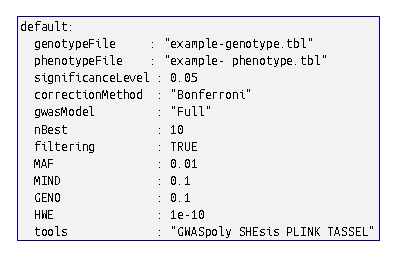
\includegraphics{images/paper-config-file}
\par\end{centering}
\caption{Configuration file for MultiGWAS. The input parameters include: the output folder where results will be written, input genotype/phenotype filenames, genome-wide significance threshold, method for multiple testing correction, GWAS model, number of associations to be reported, filtering with TRUE or FALSE whether to use quality control filters or not. The filters are: minor allele frequency, individual missing rate, SNP missing rate, and Hardy-Weinberg threshold. At the end the tools parameter defines the GWAS packages to be used for the analysis. \label{fig:Configuration-file}}
\end{figure}


\subsection{Using the command line interface}

The execution of the CLI tool is simple. It only needs to open a Linux console, change to the folder where the configuration file was created, and type the name of the executable tool followed by the the filename of the configuration file, like this:

\begin{lstlisting}[language=bash,basicstyle={\small}]
multiGWAS Test01.config
\end{lstlisting}

Then, the tool starts the execution, showing information on the process in the console window. When it finishes, the results are in a new subfolder called \emph{``out-Test01}. \lc{Cambi� ``origina graphics'' por ``source graphics''}\textcolor{blue}{{} The results include a complete HTML report containing the different views described in the results section, the source graphics and tables that support the report, and the preprocessed tables from the results generated by the four GWAS packages used by MultiGWAS.}

\subsection{Using the graphical user interface}

\textcolor{blue}{The interface allows users to save, load or specify the different input parameters for MultiGWAS in a friendly way (Fig. \ref{fig:MultiGWAS-interaction}). The input parameters correspond to the settings included in the configuration file described in the subsection \ref{section-Reading-configuration-file}.} The interface can be executed by calling the following command from a linux console:

\begin{lstlisting}[language=bash,basicstyle={\small}]
jmultiGWAS
\end{lstlisting}

\begin{figure}[H]
\begin{centering}
\includegraphics[scale=0.5]{images/paper-implementation-jmultiGWAS}
\par\end{centering}
\caption{\textbf{\textcolor{blue}{Main view of the MultiGWAS graphical user interface.}}\textcolor{blue}{{} The interface shows a main view on the center, a toolbar on the left and four tabs on top. From the main view, users can specify the input parameters for the analysis. From the toolbar, users can select the GWAS packages to be used in the analysis (two for tetraploids and two for diploids), and start the analysis with the current parameters (or load a previously saved configuration). And, from the tabs, in addition to specifying the input parameters, users can view the outputs of the process, the results of the analysis as an html report, and browse the source files that support the report.}\label{fig:MultiGWAS-interaction} }
\end{figure}


\section{Discussion}

%PAULA: Falta discutir un tris los resultados a nivel de informaci�n
%PAULA: Tools diploides vs Tools poliploides en poliploides - dosis de los alelos

XXXXXXXXXXXXXXXXXXXXXXX %Paula Consideraciones para polyploides que afectan multiGWAS requieren estudios%polyploides allele frequencies (alllele copy number). A way to solve is considering that each allele in partial heterozygotes has an equal likekihood of being present in more tahn one copy% HW polyploides autopolyploides tengo dudas si se cumple - porque la segregaci�n es diferente

Challenges studying polyploid organisms are related to the complexity of (1) the data, and (2) inheritance mechanisms that are under study (\cite{dufresne2014}). The difficulties regarding the data complexity are the uncertainty in the allele dosage and null alleles, but these problems are opportunities to improve software at the variant calling stage. Moreover, there is an on-going understanding of the inheritance mechanisms for polyploids. For autopolyploids, most loci have a polysomic inheritance. However, sections of the genome that did not duplicate lead to disomic inheritance for some loci (\cite{ohno1970,lynch2000,dufresne2014}).

MultiGWAS does not face the problem of the allele dosage uncertainty. It is necessary to measure the impact of the allele dosage uncertainty at the GWAS stage to understand the effects arisen from this problem at the association stage. However, MultiGWAS addresses the second challenge variation of inheritance mechanisms by using different for existing software: two designed for polysomic inheritance (\cite{Rosyara2016,Shen2016}) together with two for disomic inheritance (\cite{Purcell2007,Bradbury2007}). Thus it is a useful tool for researchers because it looks for significative associations that involve both types of inheritance.

%selecci�n del modelo adecuado para cada tool - %Paula: Para polyploides el modo de inheritance es complejo por eso una selecci�n del tool basada en replicabilidad y el factor de inflaci�n es una propuesta justificada
\pr{Luis esta parte revisala por fa. } Moreover, GWASpoly (\cite{Rosyara2016}) offers models for different types of polyploid gene action additive, diploidized additive, duplex dominant, simplex dominant, and general. On the other hand, TASSEL (\cite{Bradbury2007}) also models different types of gene action for diploids general, additive and dominant. We propose an automatic selection of the gene action model for both tools based on a balance between the factor of inflation and the replicability of the identified SNPs. We inform the user of the selected model based on the automatic strategy; we consider this information helps to understand the gene action model for the trait of interest. Even though the main focus is on the resultant SNPs, the model has assumptions that reflect the gene actions for a specific phenotype.

%PAULA: ventaja de integrar - pvalores inflados de shesis  (Balance entre sensitividad y especificidad al integrar)
Replicability is a strategy to assess results derived from different methods. MultiGWAS integrates results to check for replicability in the results from different software. By combining results, we can compare the outputs and look for coincidences. Some software are more sensible, and others are more specific, but the integration allows MultiGWAS to balance specificity and sensitivity.

We provide the user with different graphic outputs to help to interpret the results. We report the SNP profile for the SNPs identified by more than one software. The SNP profile gives the researcher visual feedback from the SNP. We previously check for significative SNPs based on the p-value; however, it is essential to go back to the data and check if the SNP is a real association between the genotype and phenotype. For this purpose, we designed the SNP profile. 

\section{Discussion}
\begin{enumerate}
\item For GWAS packages using several gene action models (e.g. GWASpoly and TASSEL), MultiGWAS automatically selects one of them to perform the integration with the others GWAS packages. This selection takes into account two parameters: the replicability and the inflation factor of each gene action model as at it was shown using different action model
\item Muchos de los rasgos de inter�s en las plantas est�n asociados tanto a m�ltiples genes, 
\item Cuando las herramientas diploides y tetraploides en conjunto asocian un mismo marcador al rasgo de inter�s entonces esa asociaci�n necesit� solo de la informaci�n diploide.
\end{enumerate}
\bibliographystyle{plain}
\bibliography{multiGWAS}

\end{document}
